\subsection{Algorithmes}
\begin{frame}{Algorithmes}{Ford-Fulkerson : $O(mnC^*)$}

\begin{block}{Idée générale}
\begin{itemize}
\item Trouver une chaîne améliorante.
\item Augmenter le flot le long de cette chaîne.
\end{itemize}
\end{block}

\begin{columns}
  \begin{column}[l]{0.6\textwidth}
\begin{block}{Faiblesses}
\begin{itemize}
\item "Pseudo-exponentielle" : $O(n^3)$, mais seulement pour des capacités bornées \ldots
\item "Diamant maudit" : $2\times{M}$ itérations! 
\end{itemize}
\end{block}
\end{column}
\begin{column}[l]{0.4\textwidth}
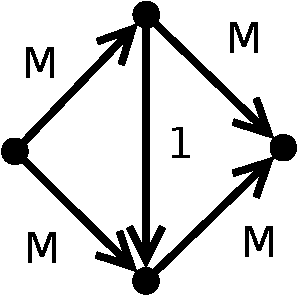
\includegraphics[width=0.5\textwidth]{img/maudit}
\end{column}
\end{columns}

\end{frame}
\begin{frame}{Algorithmes}{Edmonds-Karp : $O(n^2m)$}

\begin{block}{Idée générale}
\begin{itemize}
\item Prendre la chaîne la plus courte en nombre d'arcs
\end{itemize}
\end{block}

\begin{columns}
  \begin{column}[l]{0.6\textwidth}
\begin{block}{Faiblesses}
    \begin{itemize}
      \item Graphes avec de multiples chemins de même taille\dots
    \end{itemize}
    \end{block}
  \end{column}
 \begin{column}[r]{0.4\textwidth}
    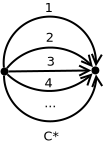
\includegraphics[width=0.5\textwidth]{img/anti_ek}
  \end{column}
\end{columns}

\end{frame}

\begin{frame}{Algorithmes}{Dinic : $O(nm^2)$}
\begin{block}{Idée générale}
\begin{itemize}
\item Rechercher l'ensemble des plus courts chemins
\item Trouver un "Flot Bloquant" dans le "Graphe de Couches"
\end{itemize}
\end{block}

\begin{columns}
  \begin{column}[l]{0.6\textwidth}

  \begin{column}[l]{0.6\textwidth}
\begin{block}{Faiblesses}
    \begin{itemize}
      \item Graphes avec de multiples chemins de plus en plus longs\dots
    \end{itemize}
    \end{block}
  \end{column}
  \end{column}
 \begin{column}[r]{0.4\textwidth}
    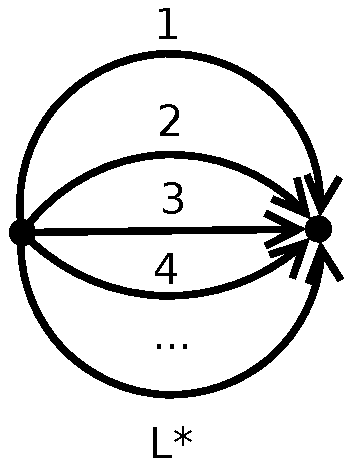
\includegraphics[width=0.5\textwidth]{img/anti_dinic}
  \end{column}
\end{columns}
\end{frame}